\DAsection[用 Commit、Branch 与 Diff 管理代码历史]{Git 核心模型与本地工作流}

\begin{frame}{2.1 Git 的三个区域}{工作区、暂存区、仓库}
  \centering
  \DAframed{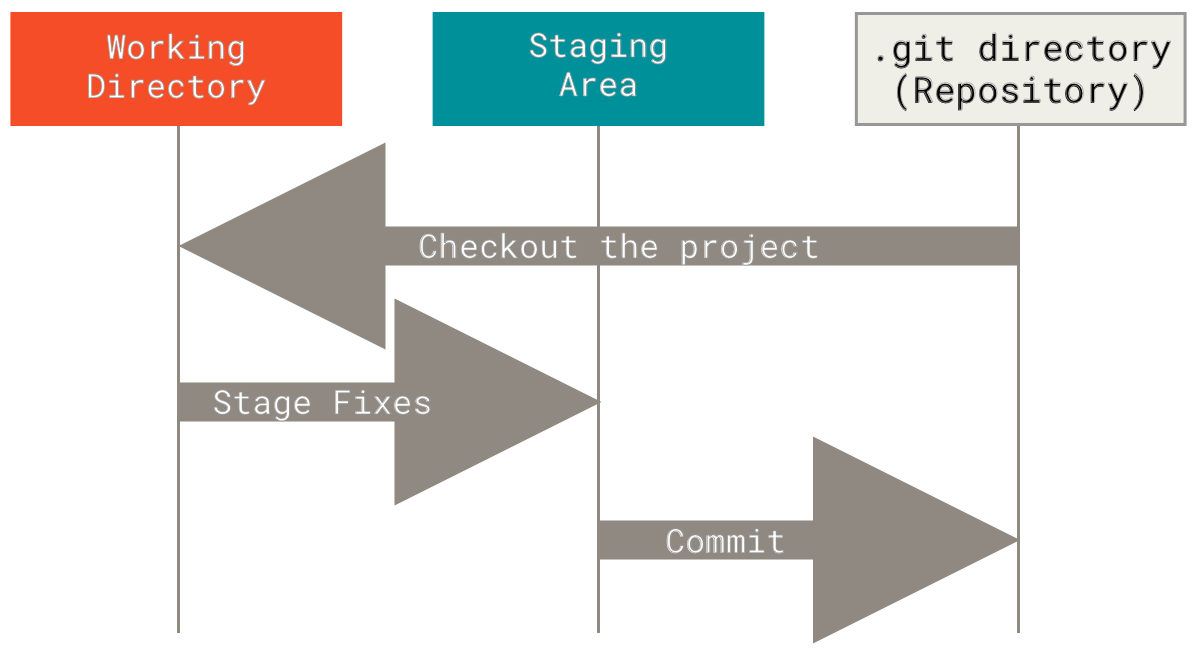
\includegraphics[width=75mm]{assets/official/collected/git-areas.png}}
  \DAtagline{关键路径}{\DAcmd{git add} 把变化送入暂存区；\DAcmd{git commit} 写入本地仓库}
  \DAsource{Pro Git · The Three States}{https://git-scm.com/book/en/v2/Getting-Started-What-is-Git\%3F}
\end{frame}

\begin{frame}[fragile]{2.2 第一次使用 Git 的身份配置}{作者信息会写入每个 Commit}
  \begin{lstlisting}[language=bash]
git config --global user.name "Your Name"
git config --global user.email "you@example.com"

git config --global init.defaultBranch main
git config --global --list
  \end{lstlisting}
  \begin{itemize}
    \item 公司与个人账号需要区分时，可在项目目录使用不带 \DAcmd{--global} 的配置。
    \item 提交邮箱应与 GitHub 账号关联，才能正确显示贡献身份。
    \item 认证使用 SSH Key 或受控 Token；密码与 Token 留在受控环境。
  \end{itemize}
\end{frame}

\begin{frame}[fragile]{2.3 获取仓库：init 与 clone}{一个创建新历史，一个复制已有历史}
  \begin{columns}[T]
    \begin{column}{0.48\textwidth}
      \begin{block}{新项目}
        \begin{lstlisting}[language=bash]
mkdir customer-service
cd customer-service
git init
git status
        \end{lstlisting}
      \end{block}
    \end{column}
    \begin{column}{0.48\textwidth}
      \begin{block}{已有项目}
        \begin{lstlisting}[language=bash]
git clone git@github.com:org/app.git
cd app
git remote -v
        \end{lstlisting}
      \end{block}
    \end{column}
  \end{columns}
  \DAtagline{团队默认}{使用 Clone 获取完整历史与远程仓库配置}
\end{frame}

\begin{frame}[fragile]{2.4 一次最小提交循环：从 git add 开始}{选择文件、检查暂存区、创建本地 Commit}
  \begin{columns}[T]
    \begin{column}{0.42\textwidth}
  \begin{lstlisting}[language=bash,basicstyle=\ttfamily\fontsize{5.4}{6.2}\selectfont]
git add docs/git-demo-notes.md
git diff --cached
git commit -m "docs: add Git workflow demo notes"
  \end{lstlisting}
      \begin{itemize}
        \item 先选择，再检查，最后提交。
        \item Commit 只写入本机仓库。
      \end{itemize}
    \end{column}
    \begin{column}{0.54\textwidth}
      \centering
      \DAframed{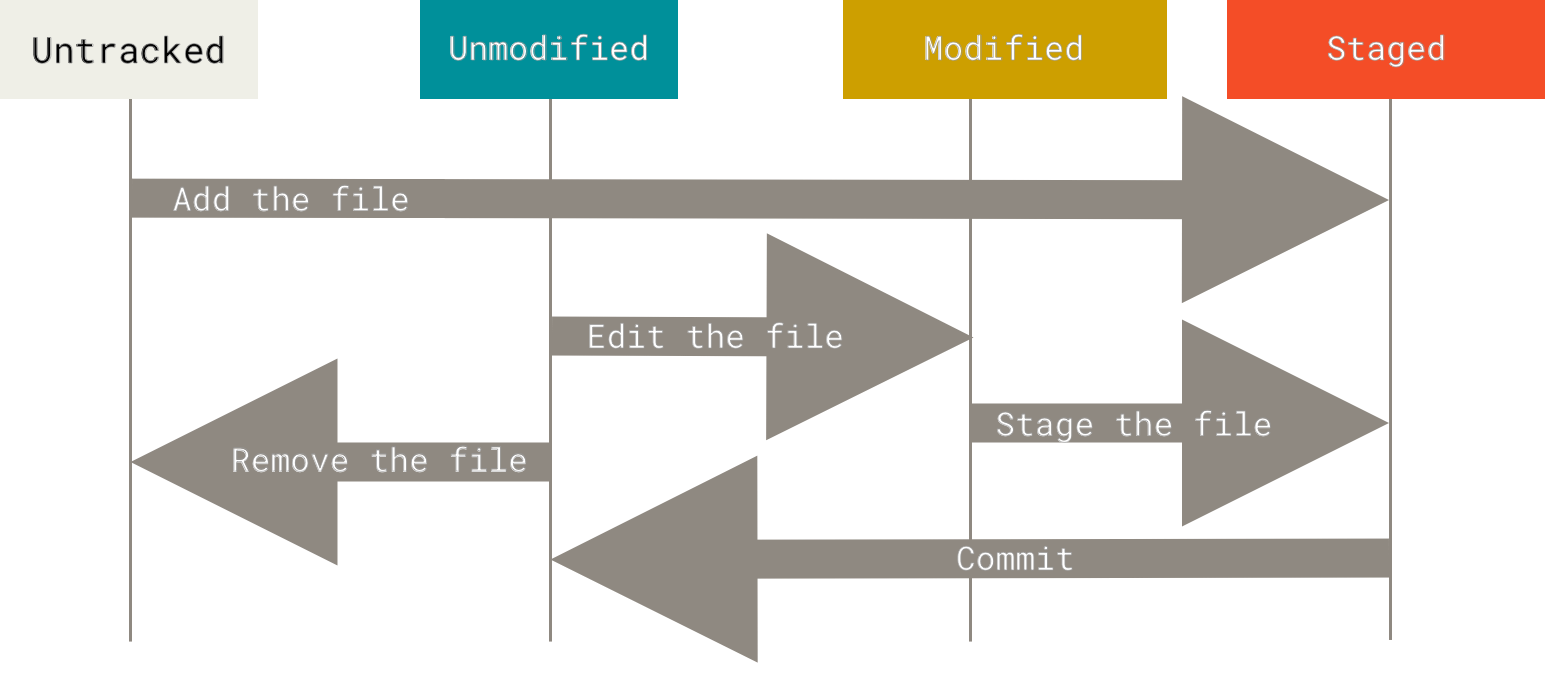
\includegraphics[width=66mm]{assets/official/collected/git-lifecycle.png}}
      \par\smallskip
      {\scriptsize 文件会在未跟踪、已修改、已暂存之间流转。}
    \end{column}
  \end{columns}
  \DAsource{Pro Git · Recording Changes}{https://git-scm.com/book/en/v2/Git-Basics-Recording-Changes-to-the-Repository}
\end{frame}

\begin{frame}[fragile]{2.5 Commit 写入本地仓库}{Commit 0fd229a}
  \begin{lstlisting}[language=bash]
$ git diff --cached --stat
 docs/git-demo-notes.md | 13 +++++++++++++
 1 file changed, 13 insertions(+)

$ git commit -m "docs: add Git workflow demo notes"
[main 0fd229a] docs: add Git workflow demo notes
 1 file changed, 13 insertions(+)
 create mode 100644 docs/git-demo-notes.md
  \end{lstlisting}
  \DAtagline{此刻}{Commit 已存在于本地，GitHub 仍停留在上一个 Commit}
\end{frame}

\begin{frame}[fragile]{2.6 Push 同步到 GitHub}{Commit 是本地动作，Push 是网络动作}
  \begin{columns}[T]
    \begin{column}{0.48\textwidth}
      \begin{block}{Push 前}
        \begin{lstlisting}[language=bash]
$ git status -sb
## main...origin/main [ahead 1]

$ git log --oneline --decorate -2
0fd229a (HEAD -> main) docs: add
  Git workflow demo notes
8ce893a (origin/main) feat: add
  deployment and operations lessons
        \end{lstlisting}
      \end{block}
    \end{column}
    \begin{column}{0.48\textwidth}
      \begin{block}{Push 后}
        \begin{lstlisting}[language=bash]
$ git push
 8ce893a..0fd229a  main -> main

$ git status -sb
## main...origin/main
        \end{lstlisting}
      \end{block}
    \end{column}
  \end{columns}
\end{frame}

\begin{frame}{2.7 好 Commit 的三个标准}{小、完整、能读懂}
  \begin{columns}[T]
    \begin{column}{0.52\textwidth}
      \begin{itemize}
        \item \textbf{单一意图}：一次只解决一个问题。
        \item \textbf{可独立验证}：提交后项目仍可运行或测试。
        \item \textbf{信息明确}：说明改了什么以及为什么改。
      \end{itemize}
      \DAtagline{示例}{\DAfile{fix(api): handle 401 response}}
    \end{column}
    \begin{column}{0.44\textwidth}
      \centering
      \DAframed{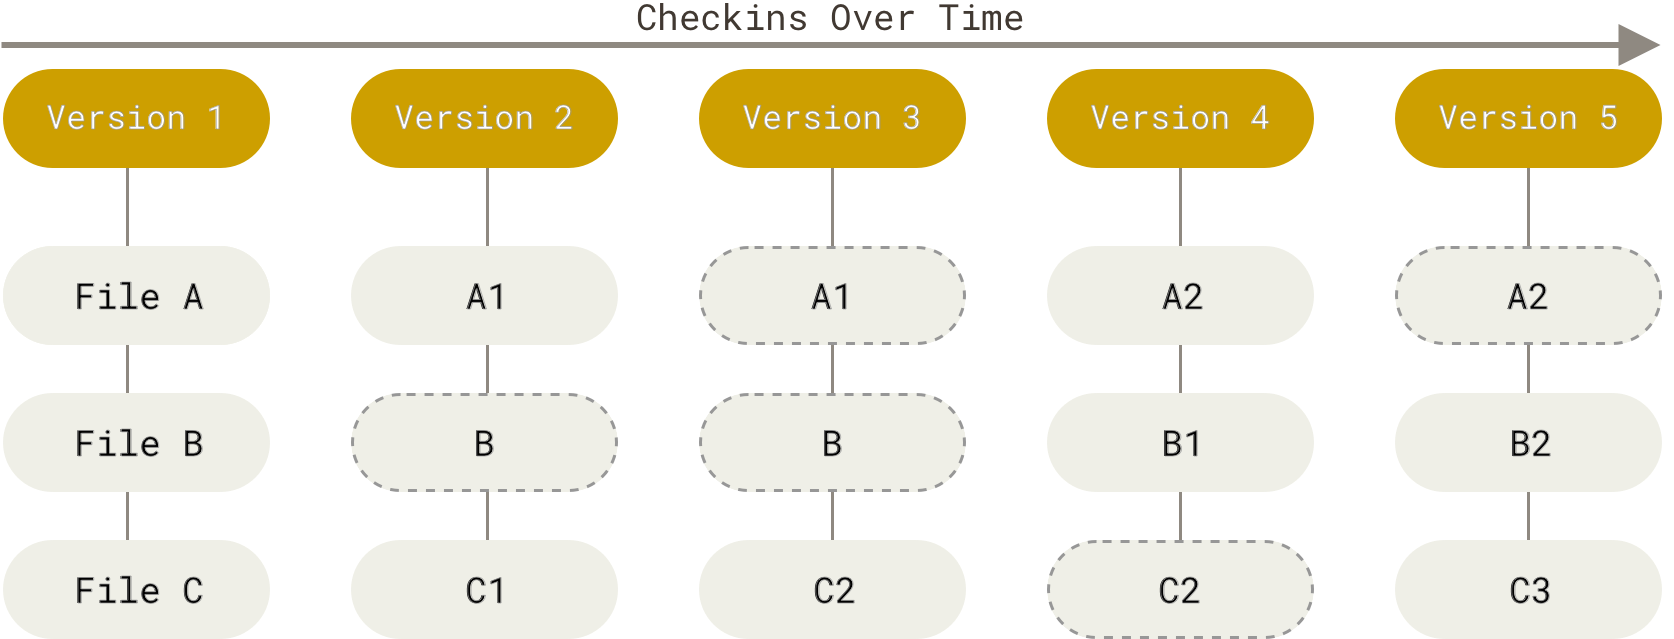
\includegraphics[width=53mm]{assets/official/collected/git-snapshots.png}}
      \par\smallskip
      {\scriptsize 每个 Commit 保存一次可追踪的项目快照。}
    \end{column}
  \end{columns}
  \DAsource{Pro Git · Snapshots, Not Differences}{https://git-scm.com/book/en/v2/Getting-Started-What-is-Git\%3F}
\end{frame}

\begin{frame}[fragile]{2.8 用 log 与 show 追踪变化}{查看提交顺序、指针位置与文件变化}
  \begin{lstlisting}[language=bash]
$ git log --oneline --decorate --graph -4
* 0fd229a (HEAD -> main, origin/main)
  docs: add Git workflow demo notes
* 8ce893a feat: add deployment and operations lessons
* bef37be feat: add Git collaboration lessons
* ab2afa2 chore: initialize Day 5 beamer project

$ git show --stat 0fd229a
 docs/git-demo-notes.md | 13 +++++++++++++
 1 file changed, 13 insertions(+)
  \end{lstlisting}
  \begin{itemize}
    \item \DAfile{HEAD -> main, origin/main} 表示本地与 GitHub 已对齐。
    \item \DAcmd{git show 0fd229a} 查看某次提交的说明与完整 Diff。
    \item \DAcmd{git diff ab2afa2..0fd229a} 比较两个历史节点。
  \end{itemize}
\end{frame}

\begin{frame}{2.9 分支是什么}{指向某个 Commit 的可移动标签}
  \centering
  \DAframed{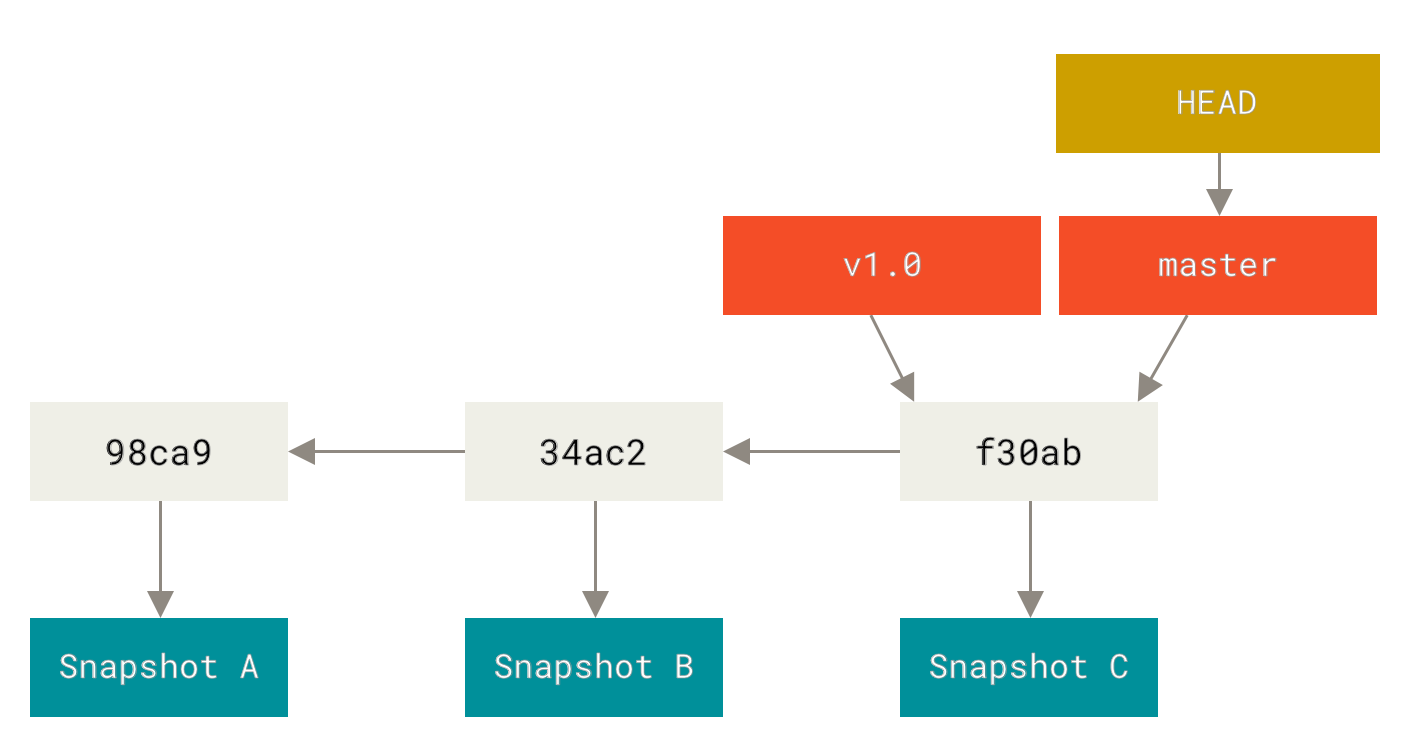
\includegraphics[width=70mm]{assets/official/collected/git-branch-history.png}}
  \begin{itemize}
    \item 分支是指向 Commit 的轻量指针。
    \item 每个任务独立分支，可以并行开发、单独 Review、随时放弃。
  \end{itemize}
  \DAsource{Pro Git · Branches in a Nutshell}{https://git-scm.com/book/en/v2/Git-Branching-Branches-in-a-Nutshell}
\end{frame}

\begin{frame}[fragile]{2.10 分支的日常命令}{从最新 main 开始工作}
  \begin{columns}[T]
    \begin{column}{0.53\textwidth}
  \begin{lstlisting}[language=bash,basicstyle=\ttfamily\fontsize{5.2}{6.0}\selectfont]
git switch main
git pull --ff-only

git switch -c feature/login-api
# edit, test, commit...

git switch main
git branch -d feature/login-api
  \end{lstlisting}
    \end{column}
    \begin{column}{0.43\textwidth}
      \centering
      \DAframed{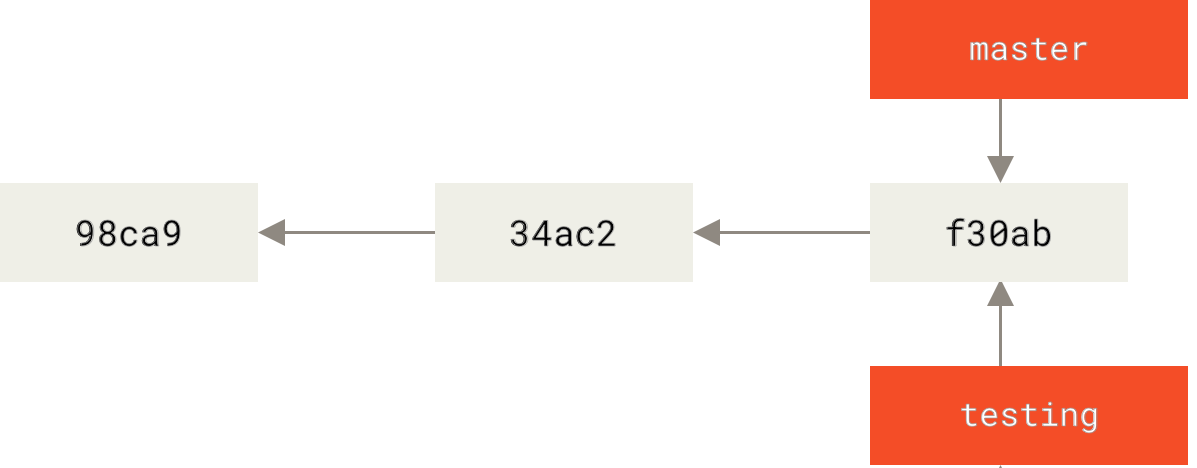
\includegraphics[width=52mm]{assets/official/collected/git-two-branches.png}}
      \begin{itemize}
        \item 从最新 \DAfile{main} 创建任务分支。
        \item 合并后及时删除过期分支。
      \end{itemize}
    \end{column}
  \end{columns}
  \DAsource{Pro Git · Basic Branching}{https://git-scm.com/book/en/v2/Git-Branching-Basic-Branching-and-Merging}
\end{frame}

\begin{frame}[fragile]{2.11 撤销操作：先判断“是否已经共享”}{公开历史优先 revert，未共享历史才考虑重写}
  \begin{DAtable*}{@{}p{29mm}p{45mm}p{47mm}@{}}
    \toprule
    场景 & 推荐命令 & 影响 \\
    \midrule
    未暂存的文件改坏 & \DAcmd{git restore file} & 丢弃本地变化 \\
    误加入暂存区 & \DAcmd{git restore --staged file} & 保留文件变化 \\
    最近 Commit 信息错 & \DAcmd{git commit --amend} & 重写未共享提交 \\
    已推送的错误 Commit & \DAcmd{git revert <commit>} & 新增反向提交，历史安全 \\
    \bottomrule
  \end{DAtable*}
  \DAtagline{红线}{共享分支不执行 \DAcmd{reset --hard} 或普通 \DAcmd{push --force}}
\end{frame}
